\documentclass[a4paper]{article}
\usepackage[a4paper,margin=0mm]{geometry}
\usepackage{fontspec}
\usepackage{unicode-math}
\usepackage{tikz}
\usepackage[table]{xcolor}
\usepackage[absolute]{textpos}
\usepackage{enumitem}
\usepackage{array}
\usepackage{multirow}

\setmainfont{Libertinus Serif}
\setsansfont{Libertinus Sans}
\setmathfont{Libertinus Math}
\newfontfamily\trackedsans{Libertinus Sans}[LetterSpace=8.0]

\definecolor{accent}{HTML}{F46530}
\definecolor{badge}{HTML}{FFBDA5}
\definecolor{ink}{HTML}{2A2E30}

\setlength{\TPHorizModule}{1mm}
\setlength{\TPVertModule}{1mm}
\setlength{\parindent}{0pt}
\pagestyle{empty}

\newcommand{\LCOL}{16mm}
\newcommand{\RCOL}{111mm}
\newcommand{\COLW}{83mm}

\newcommand{\topicheader}[2]{%
\begin{textblock*}{194mm}(16mm,10mm)
\begin{tikzpicture}
\node[fill=accent,text=white,font=\sffamily\bfseries\fontsize{13}{13}\selectfont,
      minimum width=9mm,minimum height=9mm,inner sep=0pt] at (4.5mm,-4.5mm) {#1};
\node[font=\sffamily\bfseries\fontsize{15}{16}\selectfont,text=ink,anchor=west] at (12mm,-4.5mm) {#2};
\end{tikzpicture}
\end{textblock*}
\begin{textblock*}{194mm}(16mm,22.5mm)

\begin{tikzpicture}
\fill[accent] (0,0) rectangle (194mm,0.5mm);
\end{tikzpicture}
\end{textblock*}
}

\newcommand{\pagefooter}[1]{%
\begin{textblock*}{194mm}(8mm,286.41mm)
  
\begin{tikzpicture}
    \fill[accent] (0,0) rectangle (194mm,0.6mm);
  \end{tikzpicture}
\end{textblock*}
\begin{textblock*}{63.59mm}(8mm,288.27mm)
  {\sffamily\bfseries\color{accent}\fontsize{13}{16}\selectfont SAT 1200+}
\end{textblock*}
\begin{textblock*}{10mm}(188mm,288.27mm)
  \centering{\sffamily\color{accent}\fontsize{14}{16}\selectfont #1}
\end{textblock*}
}

\newcommand{\colrule}[2]{%
\begin{textblock*}{1mm}(105mm,#1mm)
\begin{tikzpicture}
\draw[black!65,line width=0.5pt] (0,0) -- (0,#2mm);
\end{tikzpicture}
\end{textblock*}
}

\newcommand{\setkicker}[2]{%
{\sffamily\bfseries\fontsize{12}{14}\selectfont #1.}\ {\itshape\fontsize{11}{14}\selectfont\color{black!75} #2}\par\vspace{2mm}%
}

\setlength{\fboxsep}{1.4pt}
\setlength{\fboxrule}{0.5pt}
\newcommand{\pnum}[1]{\fcolorbox{ink}{white}{\sffamily\bfseries\fontsize{8}{8}\selectfont #1}~}

\newcommand{\qrbox}[1]{%
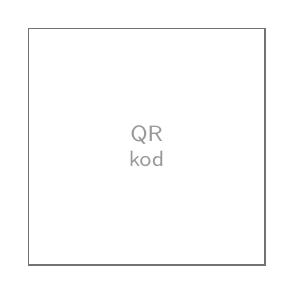
\begin{tikzpicture}
\draw[black!55,line width=0.6pt] (0,0) rectangle (30mm,30mm);
\node[black!40,font=\sffamily\fontsize{8}{9}\selectfont,align=center] at (15mm,15mm) {QR\\kod};
\end{tikzpicture}\\[1.5mm]
{\sffamily\fontsize{9}{11}\selectfont\color{black!70} #1}%
}

% ---- SAT-style multiple-choice question block: #1=number #2=stem #3-6=choices A-D ----
\newcommand{\satq}[6]{%
\noindent\pnum{#1} #2\\[2mm]
\hspace*{7mm}\begin{tabular}{@{}p{32mm}p{32mm}@{}}
(A) #3 & (B) #4 \\[2.5mm]
(C) #5 & (D) #6 \\
\end{tabular}\\[7mm]%
}

\arrayrulecolor{accent}
\setlength{\arrayrulewidth}{0.7pt}
\renewcommand{\arraystretch}{1.35}
\newcommand{\anstitle}[1]{{\sffamily\bfseries\color{accent}\fontsize{11}{13}\selectfont #1}\\[1.3mm]}

\begin{document}

% ================= PAGE 1: Set 1 | Set 2 =================
\topicheader{4}{Ishorali sonlar}
\pagefooter{27}
\colrule{32}{238}
\mbox{}%

\begin{textblock*}{\COLW}(\LCOL,32mm)
{\fontsize{12}{15}\selectfont
\setkicker{1-to'plam}{Bir xil ishorali sonlarni qo'shing.}

\noindent\pnum{1} $(-3)+(-8)=$\\[22mm]
\noindent\pnum{2} $(-15)+(-9)=$\\[22mm]
\noindent\pnum{3} $7+12=$\\[22mm]
\noindent\pnum{4} $(-20)+(-5)=$\\[22mm]
\noindent\pnum{5} $(-11)+(-14)=$\\[22mm]
\noindent\pnum{6} $25+16=$\\[22mm]
\noindent\pnum{7} $(-30)+(-12)=$\\[22mm]
\noindent\pnum{8} $9+18=$
}
\end{textblock*}

\begin{textblock*}{\COLW}(\RCOL,32mm)
{\fontsize{12}{15}\selectfont
\setkicker{2-to'plam}{Aralash ishoralar va manfiyni ayirish.}

\noindent\pnum{1} $8-(-3)=$\\[22mm]
\noindent\pnum{2} $(-5)-(-12)=$\\[22mm]
\noindent\pnum{3} $(-7)+10=$\\[22mm]
\noindent\pnum{4} $14-20=$\\[22mm]
\noindent\pnum{5} $(-9)-6=$\\[22mm]
\noindent\pnum{6} $6-(-6)=$\\[22mm]
\noindent\pnum{7} $(-18)+11=$\\[22mm]
\noindent\pnum{8} $(-4)-(-4)=$
}
\end{textblock*}

\clearpage

% ================= PAGE 2: Set 3 | Set 4 =================
\topicheader{4}{Ishorali sonlar}
\pagefooter{28}
\colrule{32}{238}
\mbox{}%

\begin{textblock*}{\COLW}(\LCOL,32mm)
{\fontsize{12}{15}\selectfont
\setkicker{3-to'plam}{Ko'paytirish va bo'lish (ikki ko'paytuvchi).}

\noindent\pnum{1} $(-6)\times7=$\\[22mm]
\noindent\pnum{2} $(-9)\times(-8)=$\\[22mm]
\noindent\pnum{3} $45\div(-5)=$\\[22mm]
\noindent\pnum{4} $(-56)\div(-7)=$\\[22mm]
\noindent\pnum{5} $12\times(-11)=$\\[22mm]
\noindent\pnum{6} $(-100)\div4=$\\[22mm]
\noindent\pnum{7} $(-13)\times(-3)=$\\[22mm]
\noindent\pnum{8} $(-81)\div(-9)=$
}
\end{textblock*}

\begin{textblock*}{\COLW}(\RCOL,32mm)
{\fontsize{12}{15}\selectfont
\setkicker{4-to'plam}{Ko'p ko'paytuvchili zanjirlar -- manfiylar sonini sanang.}

\noindent\pnum{1} $(-2)\times(-3)\times(-4)=$\\[22mm]
\noindent\pnum{2} $(-5)\times6\times(-2)=$\\[22mm]
\noindent\pnum{3} $100\div(-5)\div(-2)=$\\[22mm]
\noindent\pnum{4} $(-1)\times(-1)\times(-1)\times(-1)=$\\[22mm]
\noindent\pnum{5} $(-3)\times(-3)\times(-3)=$\\[22mm]
\noindent\pnum{6} $48\div(-4)\times(-3)=$\\[22mm]
\noindent\pnum{7} $(-10)\times(-10)\div5=$\\[22mm]
\noindent\pnum{8} $(-2)\times3\times(-4)\times(-1)=$
}
\end{textblock*}

\clearpage

% ================= PAGE 3: Set 5 | Set 6 (spot the error) =================
\topicheader{4}{Ishorali sonlar}
\pagefooter{29}
\colrule{32}{238}
\mbox{}%

\begin{textblock*}{\COLW}(\LCOL,32mm)
{\fontsize{12}{15}\selectfont
\setkicker{5-to'plam}{Qavslarni oching.}

\noindent\pnum{1} $-(9-4)+6=$\\[22mm]
\noindent\pnum{2} $-(5+3)-2=$\\[22mm]
\noindent\pnum{3} $10-(6-11)=$\\[22mm]
\noindent\pnum{4} $-(-7+2)+1=$\\[22mm]
\noindent\pnum{5} $-(8-8)-5=$\\[22mm]
\noindent\pnum{6} $3-(-4-6)=$\\[22mm]
\noindent\pnum{7} $-(12-20)-9=$\\[22mm]
\noindent\pnum{8} $-(-6-(-2))+4=$
}
\end{textblock*}

\begin{textblock*}{\COLW}(\RCOL,32mm)
{\fontsize{11}{14}\selectfont
\setkicker{6-to'plam}{Xatoni toping -- buzilgan qadamni ayting, to'g'ri javobni bering.}

\noindent\pnum{1} $8-(-3)$ ifodasida ko'rsatilgan yechimda xato bor:\\[1mm]
\hspace*{7mm}\textit{``Noto'g'ri yechim: $8-3=5$.''}\\[2mm]
\hspace*{7mm}Xato va to'g'ri javob: \makebox[52mm]{\dotfill}\\[10mm]

\noindent\pnum{2} $(-5)\times(-6)$ ifodasida ko'rsatilgan yechimda xato bor:\\[1mm]
\hspace*{7mm}\textit{``Noto'g'ri yechim: $-30$.''}\\[2mm]
\hspace*{7mm}Xato va to'g'ri javob: \makebox[52mm]{\dotfill}\\[10mm]

\noindent\pnum{3} $-(10-4)$ ifodasida ko'rsatilgan yechimda xato bor:\\[1mm]
\hspace*{7mm}\textit{``Noto'g'ri yechim: $-10-4=-14$.''}\\[2mm]
\hspace*{7mm}Xato va to'g'ri javob: \makebox[52mm]{\dotfill}\\[10mm]

\noindent\pnum{4} $(-2)\times(-2)\times(-2)$ ifodasida ko'rsatilgan yechimda xato bor:\\[1mm]
\hspace*{7mm}\textit{``Noto'g'ri yechim: barcha ko'paytuvchilar manfiy bo'lgani uchun javob musbat: $8$.''}\\[2mm]
\hspace*{7mm}Xato va to'g'ri javob: \makebox[52mm]{\dotfill}\\[6mm]

\noindent\pnum{5} $(-15)\div(-3)$ ifodasida ko'rsatilgan yechimda xato bor:\\[1mm]
\hspace*{7mm}\textit{``Noto'g'ri yechim: $-5$.''}\\[2mm]
\hspace*{7mm}Xato va to'g'ri javob: \makebox[52mm]{\dotfill}
}
\end{textblock*}

\clearpage

% ================= PAGE 4: Set 7 (bonus, left) + Set 8 pt.1 (right) -- no dead column =================
\topicheader{4}{Ishorali sonlar}
\pagefooter{30}
\colrule{32}{238}
\mbox{}%

\begin{textblock*}{\COLW}(\LCOL,32mm)
{\fontsize{12}{15}\selectfont
\setkicker{7-to'plam}{Bonus / qiyin -- har biriga taxminan 90 soniya.}

\noindent\pnum{1} $-(-8+3)\times(-2)-5=$\\[26mm]
\noindent\pnum{2} $(-4)\times(-3)-(-7)+(-2)\times5=$\\[26mm]
\noindent\pnum{3} $18\div(-3)+(-2)\times(-4)-6=$\\[26mm]
\noindent\pnum{4} $-(5-(-9))+(-14)\div7=$\\[26mm]
\noindent\pnum{5} $(-6)\times\!\left[(-2)-3\right]+(-10)\div(-5)=$
}
\end{textblock*}

\begin{textblock*}{\COLW}(\RCOL,32mm)
{\fontsize{10.5}{13}\selectfont
\setkicker{8-to'plam}{SAT'da qanday uchraydi -- harorat, balandlik, balans.}

\satq{1}{Ertalab soat 6:00 da harorat $-8°C$ edi. Peshin paytigacha harorat $15°C$ ga ko'tarildi. Peshin paytidagi harorat nechaga teng?}{$-23$}{$-7$}{7}{23}
\satq{2}{Lift $-2$-qavatdan harakatni boshlab, 9 qavat yuqoriga ko'tariladi. Lift qaysi qavatda to'xtaydi?}{$-11$}{$-7$}{7}{11}
\satq{3}{Suv osti kemasi dengiz sathidan $-120$ metr balandlikda. U yana 45 metrga sho'ng'iydi. Uning yangi balandligi nechaga teng?}{$-165$}{$-75$}{75}{165}
\satq{4}{$|{-14}|-|6|$ ifodaning qiymati nechaga teng?}{$-20$}{$-8$}{8}{20}
\satq{5}{Bank hisobida $-\$45$ balans bor. Hisob egasi $\$60$ pul qo'yadi. Yangi balans (dollarda) nechaga teng?}{$-105$}{$-15$}{15}{105}
\satq{6}{$(-7)\times(-4)\div(-2)$ ifodaning qiymati nechaga teng?}{$-14$}{$-11$}{11}{14}
}
\end{textblock*}

\clearpage

% ================= PAGE 5: Set 8 pt.2 (continues directly, no title page of its own) =================
\topicheader{4}{Ishorali sonlar}
\pagefooter{31}
\colrule{32}{238}
\mbox{}%

\begin{textblock*}{\COLW}(\LCOL,32mm)
{\fontsize{10.5}{13}\selectfont
\setkicker{8-to'plam (davomi)}{SAT'da qanday uchraydi -- harorat, balandlik, balans.}

\satq{7}{Aksiya narxi har kuni $\$3$ ga tushib boradi. 5 kun davomida narxning jami o'zgarishi (dollarda) nechaga teng?}{$-15$}{$-8$}{8}{15}
\satq{8}{$-(4-9)+(-6)$ ifodaning qiymati nechaga teng?}{$-11$}{$-1$}{1}{11}
\satq{9}{Suzuvchi dengiz sathidan $-18$ metr chuqurlikda. Uning yangi holati $-18-(-11)$ ifodasi bilan beriladi. Yangi holati nechaga teng?}{$-29$}{$-7$}{7}{29}
\satq{10}{$x=3$ bo'lganda, $-2(x-5)$ ifodaning qiymati nechaga teng?}{$-16$}{$-4$}{4}{16}
\satq{11}{To'rtta manfiy sonning ko'paytmasi olinsa, natija har doim:}{musbat bo'ladi}{manfiy bo'ladi}{musbat yoki manfiy bo'lishi mumkin}{nolga teng bo'ladi}
\satq{12}{Sayyoh $250$ m balandlikdan boshlab, $180$ m pastga, so'ngra yana $95$ m pastga tushadi. Uning hozirgi balandligi (metrda) nechaga teng?}{$-25$}{$-95$}{25}{525}
}
\end{textblock*}

\clearpage

% ================= PAGE 6: Qaydlar (notes) -- ruled writing space + video QR codes =================
\topicheader{4}{Ishorali sonlar}
\pagefooter{32}
\mbox{}%

\begin{textblock*}{194mm}(16mm,34mm)
{\bfseries\itshape\color{accent}\fontsize{19}{21}\selectfont\centering Qaydlar uchun\par}
\end{textblock*}

\begin{textblock*}{194mm}(16mm,46mm)
{\fontsize{11}{14}\selectfont\color{black!65}\centering\itshape Nimalar esingizda qoldi?\par}
\end{textblock*}

\begin{textblock*}{178mm}(16mm,62mm)
\begin{tikzpicture}
\foreach \y in {0,13,...,169}{
  \draw[black!25,line width=0.5pt] (0,-\y mm) -- (178mm,-\y mm);
}
\end{tikzpicture}
\end{textblock*}

\begin{textblock*}{194mm}(16mm,240mm)
\centering
{\sffamily\fontsize{9.5}{11.5}\selectfont\color{black!70} Video yechimlar va qo'shimcha testlar uchun quyidagi QR kodlarni skanerlang:}\\[4mm]
\begin{minipage}[t]{32mm}\centering\qrbox{YouTube}\end{minipage}%
\hspace{16mm}%
\begin{minipage}[t]{32mm}\centering\qrbox{Telegram}\end{minipage}
\end{textblock*}

\clearpage

% ================= PAGE 7: Javoblar -- single unified table =================
\topicheader{4}{Ishorali sonlar}
\pagefooter{33}
\mbox{}%

\begin{textblock*}{194mm}(16mm,30mm)
{\bfseries\itshape\color{accent}\fontsize{19}{21}\selectfont\centering Javoblar\par}
\end{textblock*}

\begin{textblock*}{194mm}(16mm,44mm)
{\fontsize{10}{12.5}\selectfont
\centering
\renewcommand{\arraystretch}{1.3}
\begin{tabular}{|>{\centering\arraybackslash}p{26mm}|>{\centering\arraybackslash}p{10mm}|>{\centering\arraybackslash}p{28mm}|>{\centering\arraybackslash}p{10mm}|>{\centering\arraybackslash}p{28mm}|}
\hline
\rowcolor{badge!55}\textbf{To'plam} & \textbf{\#} & \textbf{Javob} & \textbf{\#} & \textbf{Javob}\\
\hline
\multirow{4}{26mm}{\centering 1-to'plam} & 1 & $-11$ & 2 & $-24$\\\cline{2-5}
 & 3 & 19 & 4 & $-25$\\\cline{2-5}
 & 5 & $-25$ & 6 & 41\\\cline{2-5}
 & 7 & $-42$ & 8 & 27\\\hline
\multirow{4}{26mm}{\centering 2-to'plam} & 1 & 11 & 2 & 7\\\cline{2-5}
 & 3 & 3 & 4 & $-6$\\\cline{2-5}
 & 5 & $-15$ & 6 & 12\\\cline{2-5}
 & 7 & $-7$ & 8 & 0\\\hline
\multirow{4}{26mm}{\centering 3-to'plam} & 1 & $-42$ & 2 & 72\\\cline{2-5}
 & 3 & $-9$ & 4 & 8\\\cline{2-5}
 & 5 & $-132$ & 6 & $-25$\\\cline{2-5}
 & 7 & 39 & 8 & 9\\\hline
\multirow{4}{26mm}{\centering 4-to'plam} & 1 & $-24$ & 2 & 60\\\cline{2-5}
 & 3 & 10 & 4 & 1\\\cline{2-5}
 & 5 & $-27$ & 6 & 36\\\cline{2-5}
 & 7 & 20 & 8 & $-24$\\\hline
\multirow{4}{26mm}{\centering 5-to'plam} & 1 & 1 & 2 & $-10$\\\cline{2-5}
 & 3 & 15 & 4 & 6\\\cline{2-5}
 & 5 & $-5$ & 6 & 13\\\cline{2-5}
 & 7 & $-1$ & 8 & 8\\\hline
\multirow{3}{26mm}{\centering 7-to'plam} & 1 & $-15$ & 2 & 9\\\cline{2-5}
 & 3 & $-4$ & 4 & $-16$\\\cline{2-5}
 & 5 & 32 & -- & --\\\hline
\multirow{6}{26mm}{\centering 8-to'plam} & 1 & C & 2 & C\\\cline{2-5}
 & 3 & A & 4 & C\\\cline{2-5}
 & 5 & C & 6 & A\\\cline{2-5}
 & 7 & A & 8 & B\\\cline{2-5}
 & 9 & B & 10 & C\\\cline{2-5}
 & 11 & A & 12 & A\\\hline
\multirow{5}{26mm}{\centering 6-to'plam} & \multicolumn{4}{p{76mm}|}{1.\ Minus-minus (manfiyni ayirish) qo'shishga aylantirilmadi. To'g'ri: $8-(-3)=8+3=11$.}\\\cline{2-5}
 & \multicolumn{4}{p{76mm}|}{2.\ Bir xil ishorali ko'paytirish musbat natija beradi. To'g'ri: $(-5)\times(-6)=30$.}\\\cline{2-5}
 & \multicolumn{4}{p{76mm}|}{3.\ Manfiy ishora qavs ichidagi faqat birinchi hadga qo'llanildi. To'g'ri: $-(10-4)=-10+4=-6$.}\\\cline{2-5}
 & \multicolumn{4}{p{76mm}|}{4.\ Uchta (toq sondagi) manfiy ko'paytuvchi bor -- toq son manfiylar natijani manfiy qiladi. To'g'ri: $(-2)\times(-2)\times(-2)=-8$.}\\\cline{2-5}
 & \multicolumn{4}{p{76mm}|}{5.\ Bo'lishda ham bir xil ishora musbat natija beradi. To'g'ri: $(-15)\div(-3)=5$.}\\\hline
\end{tabular}
}
\end{textblock*}

\end{document}
